\documentclass{standalone}

\usepackage{tikz}

\definecolor{myBlue}{RGB}{56, 77, 193}

\begin{document}
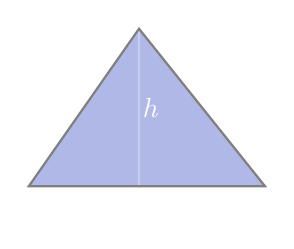
\begin{tikzpicture}
  \fill[fill=myBlue, opacity=0.4] (0,0)--(3,0)--(1.4,2);
  \node[white] at (2,-0.2) {$ b $};
  \draw[white, thick,opacity=0.3] (1.4,2)--(1.4,0);
  \node[white] at (1.55,1) {$ h $};
  \draw[color=gray,thick,opacity=1] (0,0)--(3,0)--(1.4,2)--(0,0)--(3,0);
\end{tikzpicture}	
\end{document}